\documentclass{article}
\usepackage{graphicx} % Required for inserting images
\usepackage[english]{babel}
\usepackage{amsmath}
\usepackage{amsfonts}
\usepackage{amsthm}
\usepackage{amssymb}
\usepackage{physics}
\usepackage[mathscr]{euscript}
\let\euscr\mathscr \let\mathscr\relax
\usepackage[scr]{rsfso}
\newcommand{\powerset}{\raisebox{.15\baselineskip}{\Large\ensuremath{\wp}}}


\usepackage{mathtools}


\numberwithin{equation}{section}

\newcommand{\vbh}[1]{\vb{\hat{#1}}}
\newcommand{\set}[1]{\{#1\}}
\newcommand{\FT}{\mathcal{F}}
\newcommand\perm[2][^n]{\prescript{#1\mkern-2.5mu}{}P_{#2}}
\newcommand\comb[2][^n]{\prescript{#1\mkern-0.5mu}{}C_{#2}}

\DeclareMathOperator{\spn}{span}

\makeatletter
\renewcommand*\env@matrix[1][*\c@MaxMatrixCols c]{%
  \hskip -\arraycolsep
  \let\@ifnextchar\new@ifnextchar
  \array{#1}}
\makeatother

\newtheorem{theorem}{Theorem}[section]
\newtheorem{corollary}{Corollary}[theorem]
\newtheorem{lemma}[theorem]{Lemma}

\title{PHYS 104 Homework 1}
\author{Siyu Chen}
\date{Summer 2023}

\begin{document}

\maketitle

\section{Thornton and Marion 10.9}

\paragraph{If a projectile is fired due east from a point on the surface of the Earth at a northern latitude $\lambda$ with a velocity of magnitude $v_0$ and at an angle of inclination $\alpha$, show that the lateral deflection when the projectile strikes earth is}


\begin{equation*}
    d = \frac{4 v^3_0}{g^2} \omega \sin \lambda \sin^2 \alpha \cos \alpha
\end{equation*}

Let's analyze the Earth's rotation. We have the constant rotational speed of the Earth $\dot{\theta} = \omega$, our original polar angle is $\phi_0 = \lambda$. We now move into a Cartesian coordinate with origin at the launch point and East direction as $\vbh{y}$, and the South direction as $\vbh{x}$, and the vertical upward direction as $\vbh{z}$. 

\begin{figure}[!htb]
\centering
   \begin{minipage}{0.48\textwidth}
     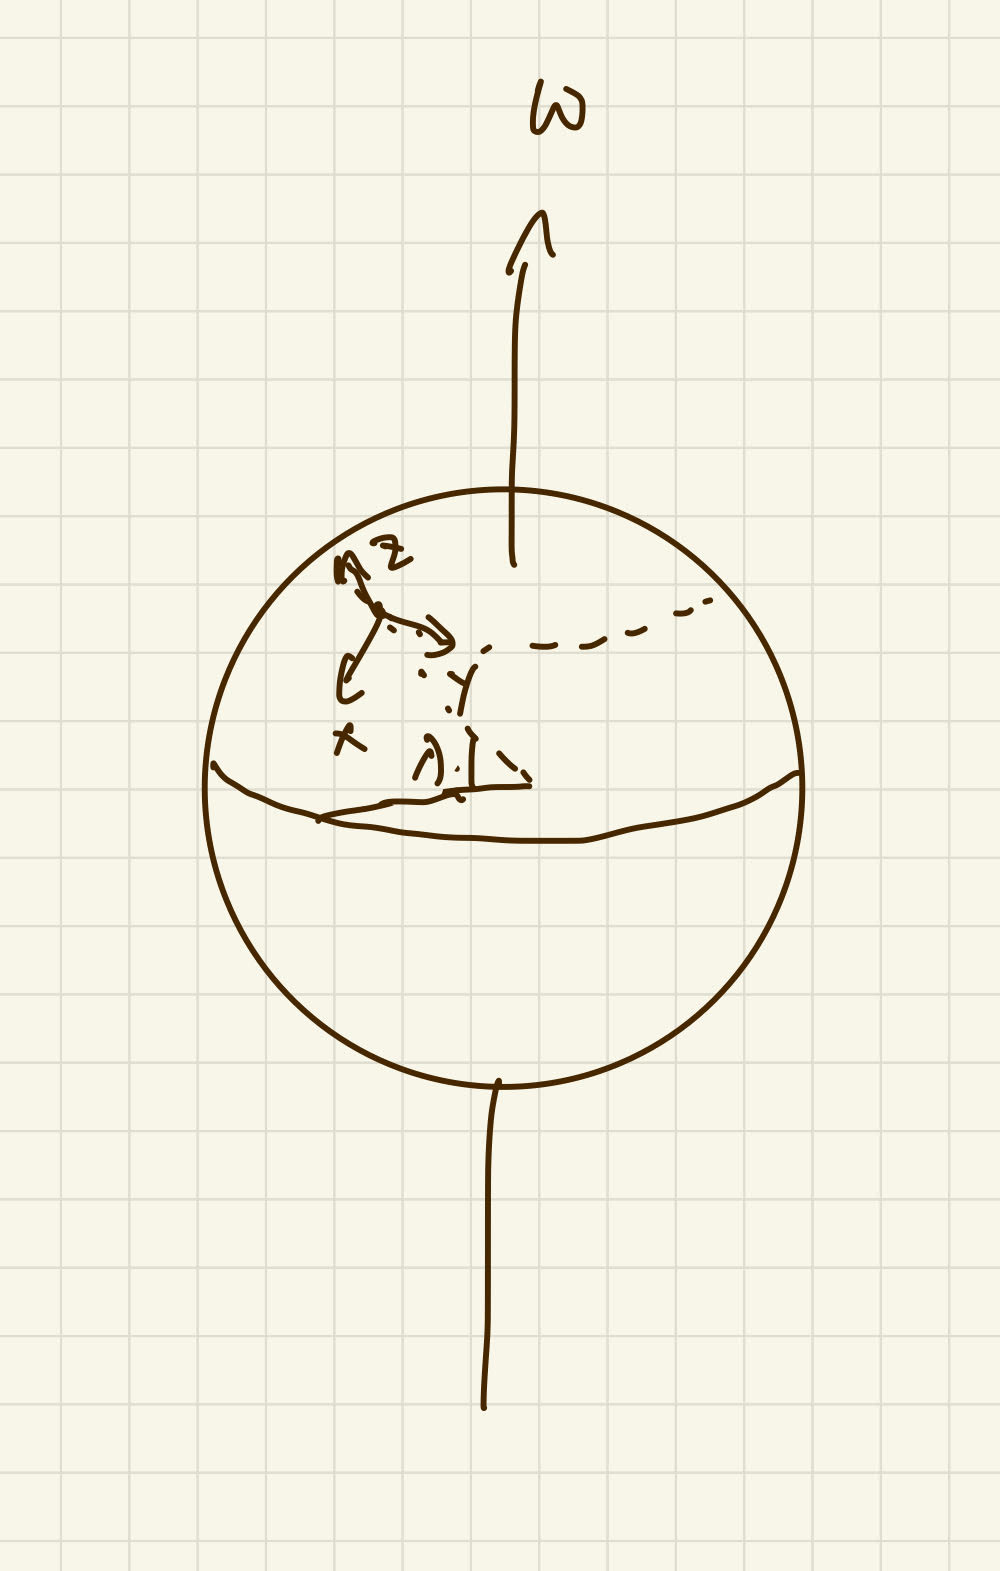
\includegraphics[width=.7\linewidth]{hw/hw1/1.1.jpg}
     \caption{Drawing of our system}
   \end{minipage}\hfill
\end{figure}

The vector for Earth's rotation points up its rotational axis, so in the new frame, we can write it as

\begin{equation}
    \va{\omega} = - \omega \cos \lambda \vbh{x} + \omega \sin \lambda \vbh{z}
\end{equation}

Our initial velocity is $\alpha$ above the horizontal. In the new frame, it can be written as:

\begin{equation}
    \va{v}_0 = v_0 \cos \alpha \vbh{y} + v_0 \sin \alpha \vbh{z}
\end{equation}

add in the acceleration of gravity to form velocity as a function of time, we have

\begin{equation}
    \va{v}(t) = v_0 \cos \alpha \vbh{y} + (v_0 \sin \alpha - gt)\vbh{z}
\end{equation}

Since our coordinate is rotating, our Coriolis force is displacing us and it is given by:

\begin{equation}
    \va{F}_{eff} = - 2m \va{\omega} \cross \va{v}_r = m \va{a}
\end{equation}

We are just interested in So our acceleration in $x$-direction as the problem asks for lateral displacement. Then our Coriolis acceleration is:

\begin{equation}
    a_x = - \lbrack 2 \va{\omega} \cross \va{v}(t) \rbrack_x = 2 v_0 \omega \cos \alpha \sin \lambda 
\end{equation}

Now, let's find the time of motion through the vertical $z$-direction:

\begin{equation}
    v_0z = g\frac{t}{2} \Rightarrow t = \frac{2v_0 \sin \alpha}{g}
\end{equation}

Notice, since the Coriolis acceleration in $z$-direction is non-zero, (1.6) is an approximation that ignores the Coriolis effect in $z$-direction. We can then assemble the kinematics equation in $x$-direction as we have the time and acceleration of the motion. We have:

\begin{equation}
    d = \frac{1}{2} a_x t^2 = \frac{4v^2_0 \sin^2 \alpha}{g^2} v_0 \omega \cos \alpha \sin \lambda = \frac{4 v^3_0}{g^2} \omega \sin \lambda \sin^2 \alpha \cos \alpha
\end{equation}

which is the expression that we were looking for.

\section{Thornton and Marion 6.9}

\paragraph{Find an expression involving the function $\phi(x_1, x_2, x_3)$ that has a minimum average value of the square of its gradient within a certain volume $V$ of space.\\}

Let $\phi(x_1, x_2, x_3)$ be our function. The average value for the square of its gradient is given by the expression:

\begin{equation}
    \frac{1}{V}\oint_V (\grad \phi)^2 dV
\end{equation}

Since our volume is given, we are trying to minimize the value of our integral. Let $f$ be a function such that:

\begin{equation}
    f = (\grad \phi )^2 = \sum_{i=1}^3 (\frac{\partial \phi}{\partial x_i})^2
\end{equation}

To minimize $f$ inside the integral, we must satisfy the Euler's equation for $f$, or the following:

\begin{equation}
     \frac{\partial f}{\partial \phi} - \frac{\partial}{\partial x_i} \frac{\partial f}{\partial \frac{\partial \phi}{\partial x_i}} = 0
\end{equation}

The first term evaluates to $0$ since $f$ is not explicitly a function of $\phi$, differentiating with respect to $\frac{\partial \phi}{\partial x_i}$ in the second term, our equation becomes:

\begin{equation}
    \sum_{i=1}^3 \frac{\partial}{\partial x_i} \frac{\partial \phi}{\partial x_i} = 0
\end{equation}

and simplifying, we have

\begin{equation}
    \grad^2 \phi = 0
\end{equation}

\section{Thornton and Marion 6.14}

\paragraph{Find the shortest path between the $(x, y, z)$ points $(0, -1, 0)$ and $(0, 1, 0)$ on the conical surface $z = 1 - \sqrt{x^2 + y^2}$. What is the length of the path?\\}

Using cylindrical coordinates, we can rewrite our conical surface as $z = 1 - r$. We can find the differential $ds$ on our path. First, in cylindrical coordinates, our $ds$ is given by

\begin{equation}
    ds = \sqrt{(dr)^2 + (dz)^2 + r^2(d\theta)^2}
\end{equation}

and since looking at our equation, we have $dz = -dr$, then (3.1) becomes:

\begin{equation}
    ds = \sqrt{ 2(dr)^2 + r^2(d\theta)^2} = \sqrt{2 + r^2 (\frac{d\theta}{dr})^2} dr
\end{equation}
 
Since the integral that we are trying to minimize is $\int_{x_0}^{x_f} ds$, the function $f = ds$ is the function whose image is the shortest path between our two points. It is a function of $r$ and $\theta$'s derivative with respect to $r$. Therefore, such function must satisfy the Euler-Lagrange equation, and we have:

\begin{equation}
    \frac{\partial f }{\partial \theta} - \frac{d}{dr} \frac{\partial f}{\partial \theta'} = 0
\end{equation}

The first term is 0 since our function does not depend on $\theta$, this means that $\frac{d}{dr}\frac{\partial f}{\partial \theta'} = 0$. Plugging in, we have:
\begin{equation}
\begin{split}
    \frac{d}{dr}(2 r\theta' (2 + r^2 \theta'^2)^{-\frac{1}{2}}) = 0
    \end{split}
\end{equation}

If we get the full description of $\theta(r)$, then we can find the path by integrating over our function. This is now a differential equation of $\theta$. Since at our initial point in cylindrical coordinates is $r = 1, \theta = -\pi/2, z = 0$ and our final point is at $r = 1, \theta = \pi /2, z = 0$, that is our boundary condition for $\theta$. We can at least see that by dimensional analysis that $\theta'$ should be the order of $1/r$. However, plugging in $\theta' = \alpha r^{-1}$ in the differentiated equation did not help. Instead, we try that:

\begin{equation}
    2 r\theta' (2 + r^2 \theta'^2)^{-\frac{1}{2}} = \text{constant}
\end{equation}

and letting that constant be $k$, we obtain

\begin{equation}
\begin{split}
(4-k) r^2 \theta'^2 = 2 k \\
4 r^2 \theta'^2 = k^2 (2+ r^2 \theta'^2)
\end{split}
\end{equation}

Simply algebraically re-arranging for $\theta'$, we have:

\begin{equation}
    \theta' = \sqrt{\frac{2k^2}{r^2(4-k^2)}}
\end{equation}

We must now use our boundary condition to figure out $k$. Integrating by separation of variable, and digging up inverse trig integral formula, we obtain:

\begin{equation}
    \theta = \sqrt{2} \sin^{-1} (\frac{k}{r}) + C
\end{equation}

Write $r$ as a function of $\theta$ and rewriting $C$ as $\phi$ as a phase shift, we have

\begin{equation}
    r = \frac{k}{\sin(\theta/\sqrt{2} - \phi)} 
\end{equation}

simply plugging the boundary condition into this does not seem to work. However, now we do have an expression with $r$ as a function of $\theta$, so let's do E.L with $\theta$ as the independent variable this time. 

\begin{equation}
    \begin{split}
        \frac{\partial f}{\partial r} - \frac{d}{d\theta} \frac{\partial f}{\partial r'} = 0
    \end{split}
\end{equation}

Writing $ds$ as $r$ yields:

\begin{equation}
    ds = \sqrt{ 2(dr)^2 + r^2(d\theta)^2} = \sqrt{2 (\frac{dr}{d\theta})^2 + r^2} d \theta
\end{equation}

I cannot figure out how to solve this differential equation, but the idea is that with a good expression, we plug in our boundary conditions to have a description of $k$ and $\phi$, and integrate $ds$ over our points and finally obtain the length. I do not know how to continue. (I saw the canvas notification way too late and tried so hard to this problem)

\section{Thornton and Marion 7.18} 
\paragraph{A pendulum is constructed by attaching a mass to an extension-less string of length $l$. The upper end of the string is connected to the uppermost point on a vertical disk of radius $R(R < l/ \pi)$. Obtain the pendulum’s equation of motion and find the frequency of small oscillations. Find the line about which the angular motion extends equally in either direction.\\}

Let's suppose that the string stays on the disk for $\theta$ angle on the disk, and since when it leaves the disk, assuming that the string is pulled tight during oscillation, the string must continue in the same direction, therefore, the angle at which the leaving string makes with the horizontal must be the same as the angle between the top of the disk, $\theta$. The arc distance that it stays on the string is $R \theta$. Let's define our origin at top of the disk. See drawing.

\begin{figure}[!htb]
\centering
   \begin{minipage}{0.48\textwidth}
     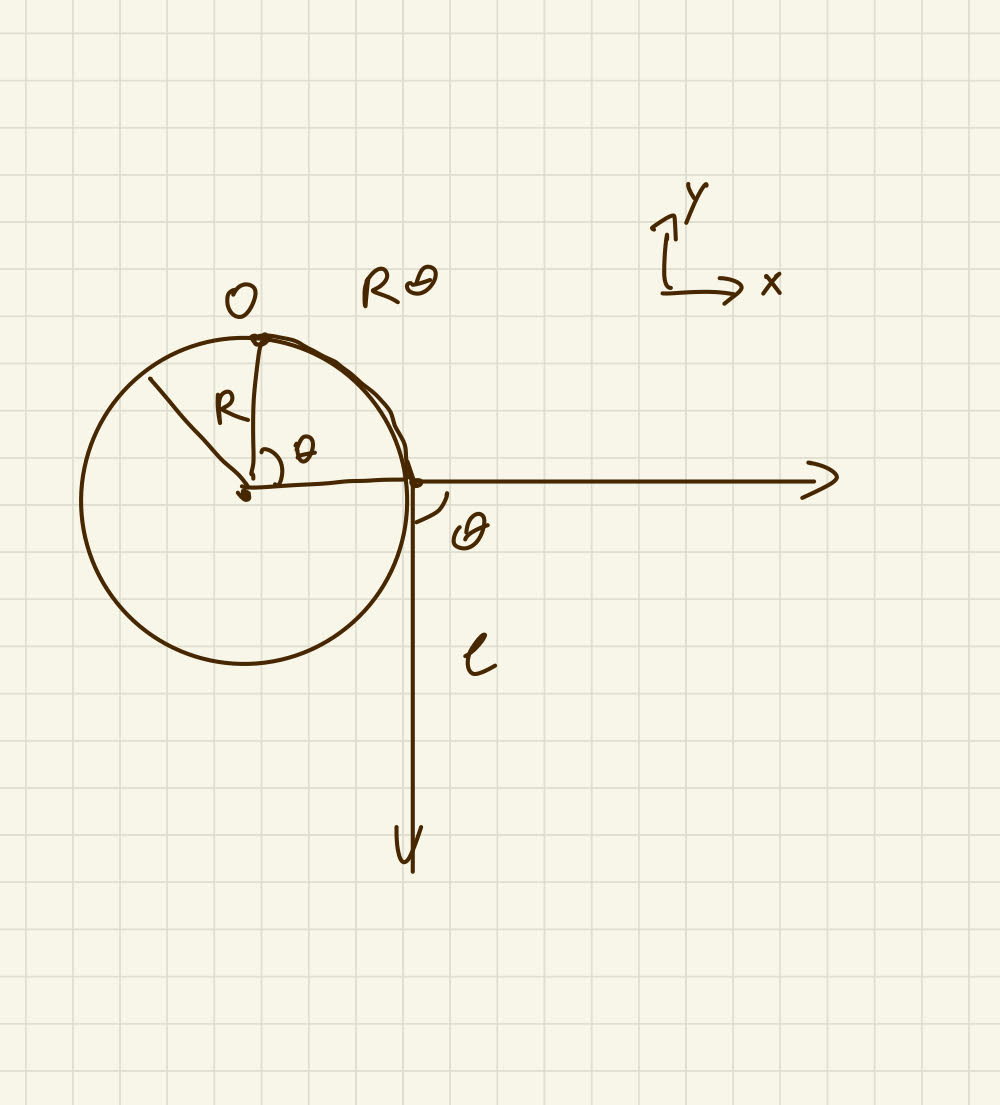
\includegraphics[width=.7\linewidth]{hw/hw1/4.1.jpg}
     \caption{Drawing of our system}
   \end{minipage}\hfill
\end{figure}


In Cartesian coordinate, we can write out the energy of our mass as the following:

\begin{equation}
\begin{split}
    T &= \frac{1}{2} m (\dot{x}^2 + \dot{y}^2) \\
    U &= mgy
\end{split}
\end{equation}

And our Lagrangian is their difference. Let's define our constraints in the Cartesian coordinate first. We have:

\begin{equation}
\begin{split}
        x &= R \sin \theta + (l - R \theta) \cos \theta \\
        y &= -R (1 -  \cos \theta) - (l - R \theta) \cos \theta
\end{split}
\end{equation}

Taking the derivatives and simplifying, we have:

\begin{equation}
\begin{split}
\dot{x} &= R \dot{\theta} \theta \sin \theta - l \dot{\theta} \sin \theta \\
\dot{y} &= R \dot{\theta} \theta \cos \theta  - l\dot{\theta} \cos \theta
\end{split}
\end{equation}

Since $R, l$ are constants, our Lagrangian would be a function of $\theta, \dot\theta$ with independent variable of time. This means that our constraint was holonomic and it eliminated one degree of freedom. Plugging in our results from (4.3) and (4.2) into (4.1), we have our Lagrangian:

\begin{equation}
    L = \frac{1}{2} m(l^2 \dot{\theta}^2 + R^2 \theta^2 \dot\theta^2 - 2Rl\theta \dot{\theta}^2) + mg ((l - R \theta) \sin\theta - R \cos \theta) 
\end{equation}

Evaluating it in Euler-Lagrange equation and simplifying, we have

\begin{equation}
    \begin{split}
        \frac{\partial L}{\partial \theta} &- \frac{d}{dt} \frac{\partial L}{\partial \dot{\theta}} = 0 \\
        g \cos \theta &= (l - R \theta )\ddot{\theta} - R \dot{\theta}^2
    \end{split}
\end{equation}

Since $\theta$ is small, we can write $\cos \theta = 1 - \theta^2 / 2$. We have in the original equation:

\begin{equation}
    (l-R \theta) \ddot{\theta} - R \dot{\theta}^2 + g\theta^2 / 2 = g
\end{equation}

where the solution to this differential equation would be our answer, but even with such approximation, I do not know how to solve the differential equation. The question also asks us to find an angle in which the angular motion extends in both directions equally, which would be the equilibrium of this oscillation. So oscillation around that equilibrium angle could be considered small. Let \begin{equation}
    \phi = \theta - \theta_0
\end{equation}

and consider this displacement of angle to be small. We can then approximate $\cos (\phi + \theta_0)$:

\begin{equation}
    \cos(\phi+\theta_0) = \cos \theta_0 \cos \phi + \sin \theta_0 \sin \phi
\end{equation}

If we eliminate all second order $\phi$ terms, i.e, $\sin \phi = \phi, \cos \phi = 1$, we have

\begin{equation}
    \cos(\phi + \theta_0) = \cos \theta_0 + \phi \sin \theta_0
\end{equation}

In the original equation (4.5), we have

\begin{equation}
    g(\cos\theta_0 + \phi \sin \theta_0) = (l-R\theta_0) \ddot{\theta} - R\dot{\theta}^2
\end{equation}

but if we say that$\ddot{\phi} = \ddot{\theta}$ and that $\dot{\theta}^2$ is also a second order term of $\phi$, and ignore that term, we have:

\begin{equation}
    g(\cos \theta_0 + \phi \sin \theta_0) = (l - R \theta_0) \ddot{\phi}
\end{equation}

solving this differential equation (I did not do it by hand), we have:

\begin{equation}
    \phi = C \sin(\sqrt{\frac{g \sin \theta_0}{l-R \theta_0}}t + \Omega) + \cot \theta_0
\end{equation}

Where $\Omega$ is a phase shift. Since we want this to be a simple oscillation, we take $\cot \theta_0 = 0$, which means that $\theta_0 = \pi/2$, and $\sin\theta_0 = 1$, we can write our equation again:

\begin{equation}
    \phi = C \sin (\sqrt{\frac{g}{l-R \theta_0}} t + \Omega)
\end{equation}

Our angular frequency is $\omega = \sqrt{\frac{g}{l-R \theta_0}}$ and the line of equilibrium oscillation extends at $\theta_0 = \pi /2$, which is to be expected since that is where our string hangs vertically downward from our disk. 

\section{Thornton and Marion 7.27} 

\paragraph{A massless spring of length $b$ and spring constant $k$ connects two particles of masses $m_1$ and $m_2$. The system rest of a smooth table and may oscillate and rotate. Write down Lagrange’s equations of motion and identify the generalized momenta associated with any cyclic coordinates. \\}


Write down the energy terms for our system in Cartesian coordinates, we have:

\begin{equation}
    \begin{split}
        T &= \frac{1}{2} m_1(\dot{x_1}^2 + \dot{y_1}^2) + \frac{1}{2} m_2(\dot{x_2}^2 + \dot{y_2}^2) \\
        U &= \frac{1}{2} k((x_1-x_{i1})^2 + (y_1-y_{i1})^2) + \frac{1}{2} m((x_2-x_{i2})^2 + (y_2-y_{i2})^2) \\
        L &= T - U
    \end{split}
\end{equation}

Let us set the coordinate of one particle as the origin in the polar coordinate for the other particle. The other one is fixed by a length of $r$, which is variable to $b$; across the horizontal is our angle $\theta$. $x_2$ becomes:

\begin{figure}[!htb]
\centering
   \begin{minipage}{0.48\textwidth}
     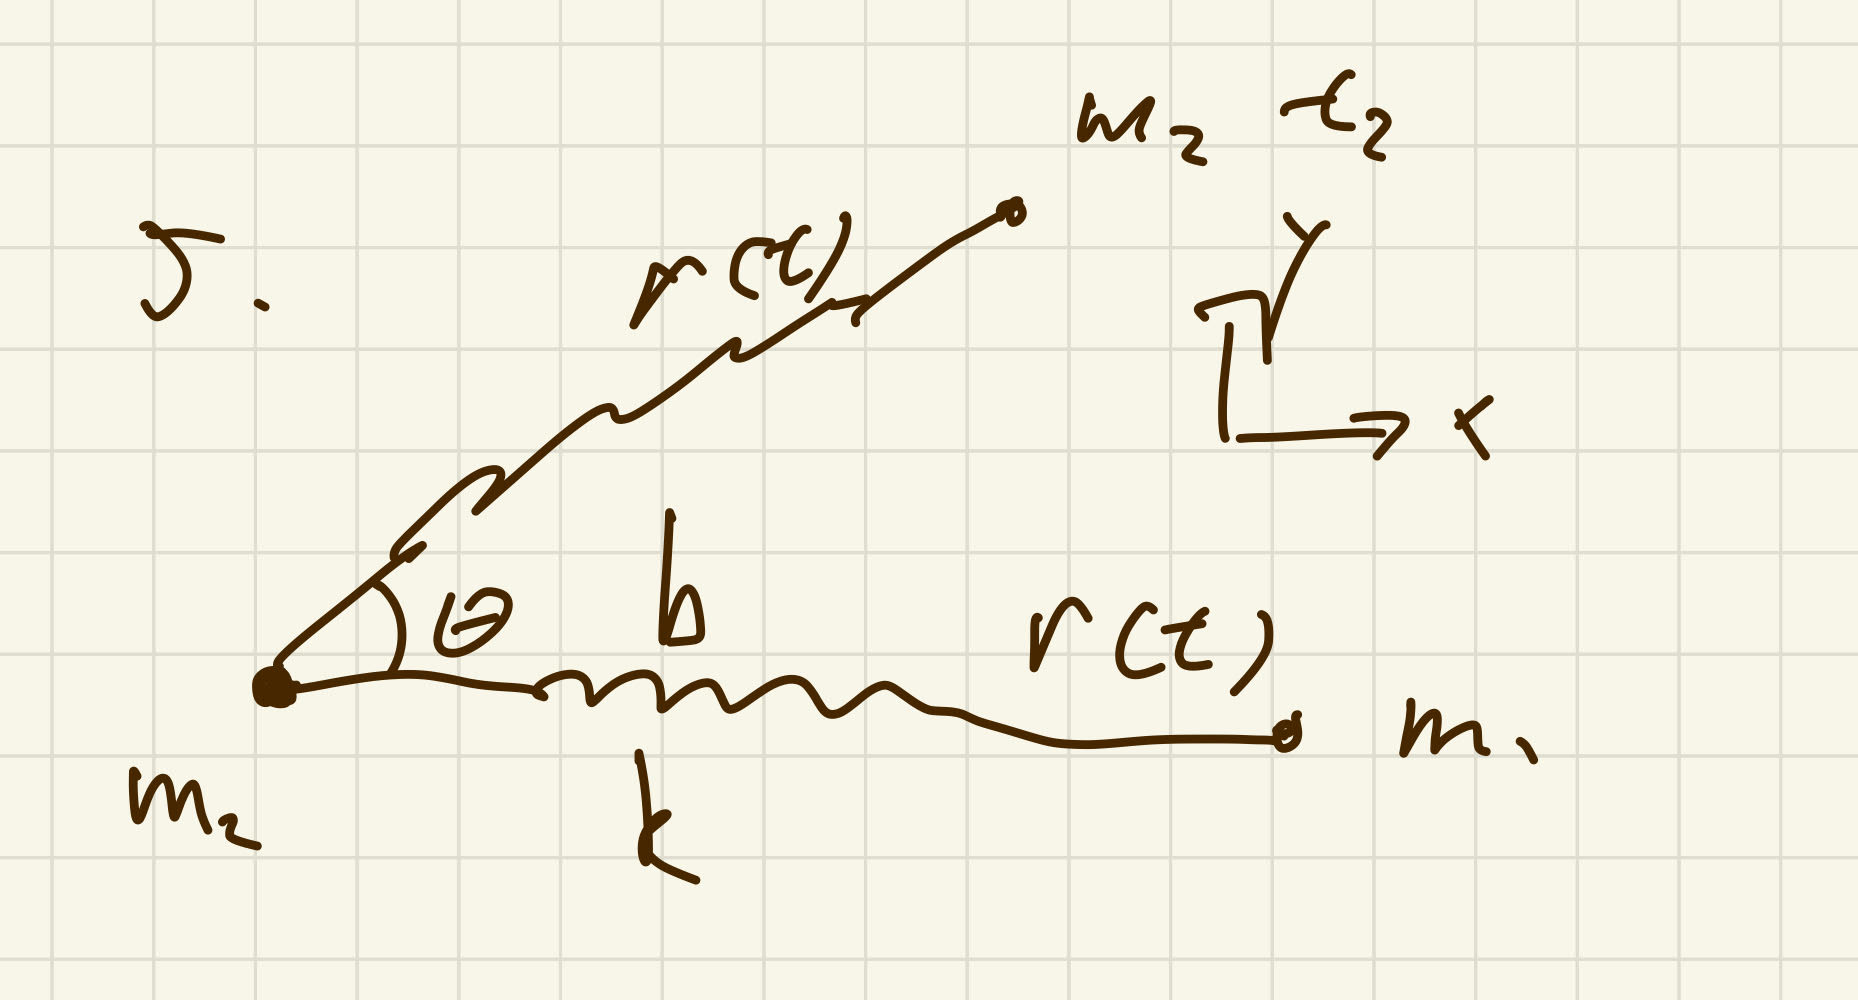
\includegraphics[width=.7\linewidth]{hw/hw1/5.1.jpg}
     \caption{Drawing of our system}
   \end{minipage}\hfill
\end{figure}

\begin{equation}
\begin{split}
        x_2 &= x_1 + r \cos \theta \\
        y_2 &= y_1 + r \sin \theta
\end{split}
\end{equation}

Their derivatives are:

\begin{equation}
    \begin{split}
        \dot{x_2} &= \dot{x_1} + \dot{r} \cos \theta - r \dot\theta \sin \theta  \\
        \dot{y_2} &= \dot{y_1} + \dot{r} \sin \theta + r \dot\theta \cos \theta 
    \end{split}
\end{equation}

our kinetic energy for the second particle becomes:

\begin{equation}
\begin{split}
        T_2 &= \frac{1}{2}m_2 (x^2_2 + y^2_2) \\
        T_2 &= \frac{1}{2} m_2 \lbrack (\dot{x_1} + \dot{r} \cos \theta - r \dot\theta \sin \theta)^2 + (\dot{y_1} + \dot{r} \sin \theta + r \dot\theta \cos \theta )^2 \rbrack //
\end{split}
\end{equation}

and our Lagrangian becomes:

\begin{equation}
\begin{split}
        T &= \frac{1}{2} m_1(\dot{x_1}^2 + \dot{y_1}^2) +   T_2(r, \dot{r}, \theta, \dot\theta, \dot{x}, \dot{y})\\
        U &= \frac{1}{2} kr^2 \\
        L &= \frac{1}{2} m_1(\dot{x_1}^2 + \dot{y_1}^2) +   T_2(r, \dot{r}, \theta, \dot\theta, \dot{x}, \dot{y}) - \frac{1}{2} kr^2
\end{split}
\end{equation}

We represent the second particle in $r, \theta$, so there are 4 degrees of freedom and two of them express the second particle in this polar coordinate way. The complete Euler-Lagrange equations of this system is:

\begin{equation}
    \begin{split}
        \frac{\partial L}{\partial x_1} - \frac{d}{dt} \frac{\partial L}{\partial \dot{x_1}} &= 0 \\ 
        \frac{\partial L}{\partial y_1} - \frac{d}{dt} \frac{\partial L}{\partial \dot{y_1}} &= 0 \\ 
        \frac{\partial L}{\partial r} - \frac{d}{dt} \frac{\partial L}{\partial \dot{r}} &= 0 \\ 
        \frac{\partial L}{\partial \theta} - \frac{d}{dt} \frac{\partial L}{\partial \dot{\theta}} &= 0 \\ 
    \end{split}
\end{equation}

Where $L$ is defined above. Since $L$ is not a function of $x, y$, the position of our first particle, necessarily, our system is invariant to translation of our first particle, which would translate the entire system since the second particle is connected by it. Therefore, in our Euler-Lagrange equation, we can see that $\frac{\partial L}{\partial x} = \frac{\partial L}{\partial y} = 0$. This means that $\frac{\partial L}{\partial \dot{x}}, \frac{\partial L}{\partial \dot{y}}$ are constants, or:

\begin{equation}
\begin{split}
        \frac{\partial L}{\partial x_1} &= m_1x_1 + m_2 (\dot{x_1} + \dot{r} \cos \theta - r \dot\theta \sin \theta) = m_1 \dot{x_1} + m_2 \dot{x_2} = \text{constant} \\
    \frac{\partial L}{\partial y_1} &= m_1y_1 + m_2 (\dot{y_1} + \dot{r} \sin \theta - r \dot\theta \cos \theta) = m_1 \dot{y_1} + m_2 \dot{y_2} =\text{constant}
\end{split}
\end{equation}

We can reasonably expect that our translation symmetry in our Lagrangian leads to a conservation of general momenta, and since these are the only properties conserved, $m_1 \dot{x_1} + m_2 \dot{x_2},  m_1 \dot{y_1} + m_2 \dot{y_2}$ are the general momenta that we are looking for for this system. Now let's compute the full Lagrangian for all four coordinates. The first two, $x_1, y_1$ we have done already, we can just use our previous result:

\begin{equation}
\begin{split}
     \frac{d}{dt} (m_1 \dot{x_1} + m_2 \dot{x_2}) &= 0 \\
     \frac{d}{dt} (m_1 \dot{y_1} + m_2 \dot{y_2}) &= 0 \\
\end{split}
\end{equation}

Notice that we can word this in the same way in (5.7), it is equivalent. And $\dot{x_2}, \dot{y_2}$ are defined in (5.3) and would be more complicated to take time derivative, but this should be a satisfactory form. Let's continue to $r, \theta$. Since these terms are more complicated, for clarity, I will write individual partial derivatives out before putting them in the full equations. We have:

\begin{equation}
    \begin{split}
        \frac{\partial L}{\partial r} &= m_2 \dot{x_2} \dot{\theta} \sin \theta + m_2 \dot{y_2} \dot{\theta} \cos \theta - kr \\
        \frac{\partial L}{\partial \dot{r}} &= m_2 \dot{x_2} \cos \theta + m_2 \dot{y_2} \sin \theta \\
        \frac{\partial L}{\partial \theta} &=  m_2 \dot{x_2}( - \dot{r} \sin \theta - r \dot{\theta} \cos \theta) + m_2 \dot{y_2}( \dot{r} \cos\theta - r \dot{\theta} \sin \theta) \\
        \frac{\partial L}{\partial \dot{\theta}} &= m_2 \dot{x_2} (- r \sin \theta) + m_2 \dot{y_2} (r \cos \theta)
    \end{split}
\end{equation}

So for the last two Euler-Lagrange Equations, we have:

\begin{equation}
\begin{split}
    (m_2 \dot{x_2} \dot{\theta} \sin \theta + m_2 \dot{y_2} \dot{\theta} \cos \theta - kr) - \frac{d}{dt}(m_2 \dot{x_2} \cos \theta + m_2 \dot{y_2} \sin \theta) &= 0 \\
    (m_2 \dot{x_2}( - \dot{r} \sin \theta - r \dot{\theta} \cos \theta) + m_2 \dot{y_2}( \dot{r} \cos\theta - r \dot{\theta} \sin \theta))&\\ - \frac{d}{dt} \lbrack m_2 \dot{x_2} (- r \sin \theta) + m_2 \dot{y_2} (r \cos \theta) \rbrack &= 0
\end{split}
\end{equation}

\end{document}
